\documentclass[spanish]{beamer}

%Language symbols
\usepackage[spanish]{babel}
\selectlanguage{spanish}
\usepackage[utf8]{inputenc}
\usepackage{verbatim}


\usepackage{graphicx}% http://ctan.org/pkg/graphicx
\usepackage{caption,subcaption}

% Code

\usepackage{listings,textcomp}
\lstset{
  breakatwhitespace,
  language=c++,
  columns=fullflexible,
  keepspaces,
  breaklines,
  tabsize=2, 
  showstringspaces=false,
  extendedchars=true,
  basicstyle=\fontfamily{pcr}\selectfont\scriptsize,
  keywordstyle=\color{orange},
  upquote=true,
  literate={-}{-}1}

%Theme
\usetheme{metropolis}

%Title
\title{Análisis de la eficiencia de algoritmos}
\date{\today}
\author{Yábir G. Benchakhtir}
\institute{Doble Grado en Ingeniería Informática y Matemáticas}
%Document
\begin{document}

\frame{\titlepage}

\begin{frame}\frametitle{Algoritmos de ordenación $O(n^2)$}

  \begin{itemize}
  \item Burbuja
  \item Insercción
  \item Selección
  \end{itemize}
\end{frame}

%
%======================
%

\begin{frame}\frametitle{Algoritmo burbuja}
  \begin{figure}[H]
    \centering   
        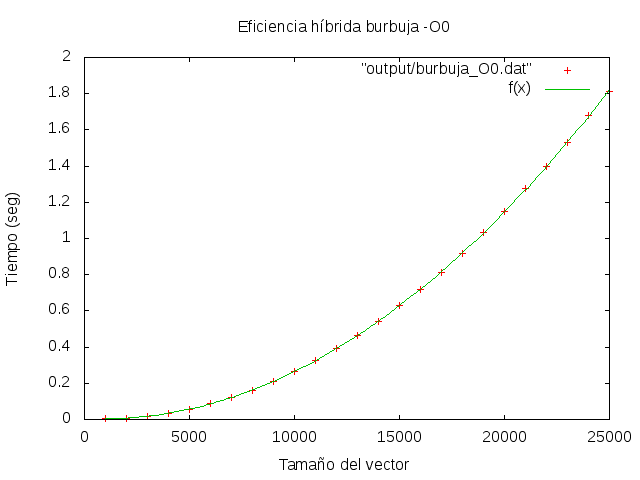
\includegraphics[clip,width=1\columnwidth]{../../plots/burbuja_O0_fit.png}%
    \end{figure}
  \end{frame}

\begin{frame}[fragile]
  Para su ajuste he usado la función:

  $$ax^2+bx+c$$

  Con ello obtenemos una bondad del ajuste de:
  
\begin{verbatim}
prueba
\end{verbatim}
  
\end{frame}


%
%======================
%

\begin{frame}\frametitle{Algoritmo de insercción}
  \begin{figure}[H]
    \centering   
        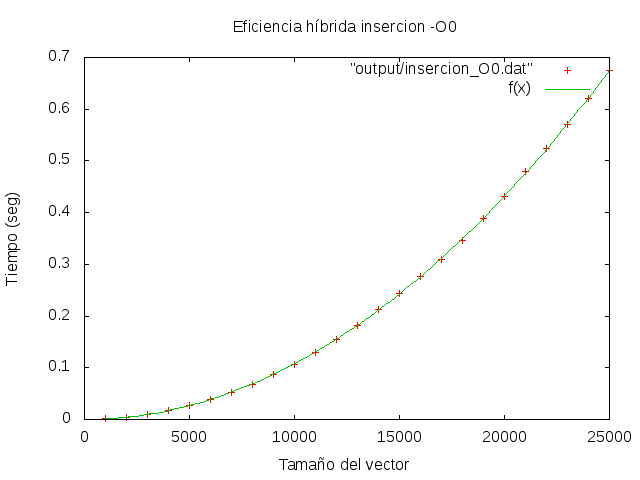
\includegraphics[clip,width=1\columnwidth]{../../plots/insercion_O0_fit.png}%
    \end{figure}
  \end{frame}

\begin{frame}[fragile]
  Para su ajuste he usado la función:

  $$ax^2+bx+c$$

  Con ello obtenemos una bondad del ajuste de:
  
\begin{verbatim}
prueba
\end{verbatim}
  
\end{frame}

%
%======================
%

\begin{frame}\frametitle{Algoritmo de selección}
  \begin{figure}[H]
    \centering   
        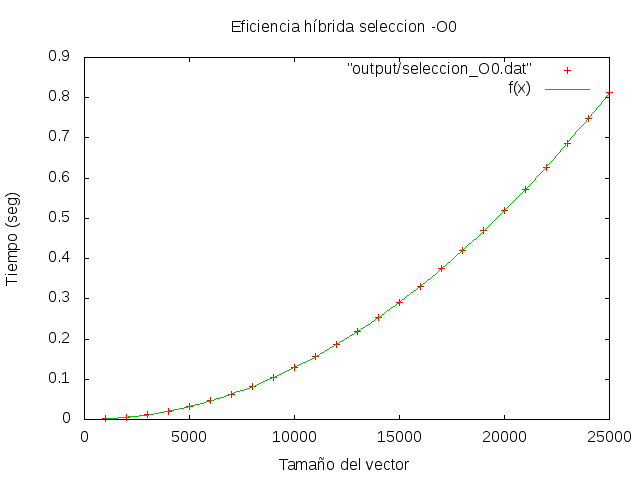
\includegraphics[clip,width=1\columnwidth]{../../plots/seleccion_O0_fit.png}%
    \end{figure}
  \end{frame}

\begin{frame}[fragile]
  Para su ajuste he usado la función:

  $$ax^2+bx+c$$

  Con ello obtenemos una bondad del ajuste de:
  
\begin{verbatim}
prueba
\end{verbatim}
  
\end{frame}

%
%======================
%

\begin{frame}\frametitle{Comparación de los algoritmos}
  \begin{figure}[H]
    \centering   
        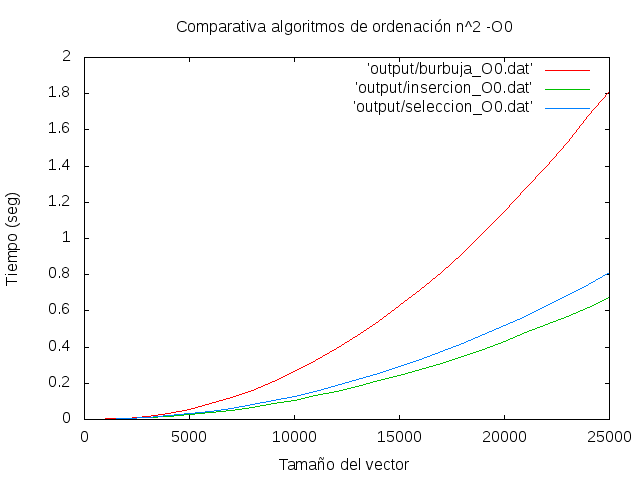
\includegraphics[clip,width=1\columnwidth]{../../plots/cuadraticos_O0.png}%
    \end{figure}
  \end{frame}

\end{document}